\documentclass[12pt]{article}
\usepackage{graphicx}
\usepackage[utf8]{inputenc}
\usepackage[german]{babel}
\usepackage{hyperref}
\usepackage{float}



\title{Pflichtenheft \\
Binding of Newton}
\author{Gabriel Goller, Tobias Kofler, Max Molling, \\
Lukas Oberhauser, Johannes Stafler}

\begin{document}
\begin{titlepage}
\maketitle
\end{titlepage}


\begin{center}
\begin{tabular}{ | c | c | c | c | } 
\hline
Version & Datum & Autor & Bemerkung\\ 
\hline
1.1 & 20.April & Max Molling & Ersterstellung\\ 
\hline
1.2 & 25.April & Max Molling & Fertigstellung\\ 
\hline
1.3 & 25.April & Gabriel Goller & Formatierung und Diagramme\\ 
\hline
\end{tabular}
\end{center}






\tableofcontents


\section{Einleitung}
\subsection{Allgemeines}
\subsubsection{Zweck und Ziel dieses Dokuments}
Dieses Pflichtenheft beschreibt die Planung der Software, die Rollenverteilung im Team und den geplanten Zeitablauf. Das Pflichtenheft gibt außerdem den Verwendungszweck der Software wieder. 

\subsection{Verteiler}
\subsubsection{Verteiler für dieses Lastenheft}


\begin{center}
\begin{tabular}{ | c | c | } 
\hline
Rolle / Rollen $\ast$ & Name \\
\hline
Programmierer & Gabriel Goller \\
\hline
Projektleiter & Tobias Kofler \\
\hline
Programmierer & Tobias Kofler \\
\hline
Designer & Max Molling \\
\hline
Schnittstelle Design-Code & Lukas Oberhauser \\
\hline
Design & Johannes Stafler \\
\hline
Zuständig für die Dokumentation & Johannes Stafler \\
\hline
\end{tabular}
\end{center}


$\ast$ Die Rollen verstehen sich als grobe Einteilung, es kann auch zu Überschneidungen zwischen den Rollen kommen.


\subsection{Ziele des Anbieters}
Es soll ein Spiel Entwickelt werden was der Top-Down Kategorie angehört.\\
Das Spiel soll folgende allgemeine Kriterien erfüllen:\\
- Eine angemessene Benutzeroberfläche für Benutzer anbieten.\\
- Eine angemessene Art der Datenspeicherung anbieten.\\
- Eine Story beinhalten, welche auf wichtigen Wissenschaftliche Ereignisse basiert

\subsection{Benutzer / Zielgruppe}
Das Spiel wird für den Auftraggeber Larcher GmbH entwickelt.

\subsection{Systemvoraussetzungen}
Für den Betrieb der Software ist keine bestimmte Hardware vorgesehen. Die Software muss allerdings kompatibel sein mit Microsoft Windows 7 oder höher und/oder einem vergleichbaren oder moderneren Betriebssystem.

\section{Allgemeine Informationen zum Spiel}
\subsection{Performanz}
Die Software muss unter vom Auftragnehmer vorgeschlagenen Mindestvoraussetzungen oder so laufen, dass alle funktionalen und nicht-funktionalen Anforderungen stets erfüllt werden. Insbesondere muss die Software die Bedingungen unter Punkt 2.7 erfüllen.

\subsection{Look and Feel}
Das Navigieren durch die GUI der Software soll dem „Look and Feel$``$-Prinzip folgen. Es ist dem Auftragnehmer überlassen, wie dies erreicht wird. Neben der Funktionalität ist es besonders wichtig, dass ein Benutzer mit der Software schnell zurechtkommt.

\subsection{Software-Ergonomie}
Die Software soll sich so weit als möglich an die Norm DIN EN ISO 9241\  halten. Diese Norm spezifiziert das angenehme und intuitive Arbeiten mit Software. Vor allem soll die GUI den Richtlinien in dieser Norm entsprechen und dem User eine moderne und leicht verständliche Oberfläche bieten.

\subsection{Portabilität}
Die vorgegebene Programmiersprache Java ermöglicht bereits ein hohes Maß an Portabilität. Der Auftragnehmer ist dazu verpflichtet die Software in mindestens zwei verschiedenen Betriebssystemen zu testen. 

\subsection{Datensicherheit}
- Benötigte Daten werden in Textdateien gespeichert. Das Format kann frei gewählt werden, empfohlen wird das CSV-System (Comma Separated Values). Die Daten können auch in einer  Datenbank gespeichert werden.\\
- Die gespeicherten Daten sind nach Möglichkeit des Auftragnehmers abzusichern.\\
- Alle dem Auftragnehmer möglichen Sicherheitsmaßnahmen sind zu treffen.

\subsection{Wartbarkeit}
Die Software muss so gestaltet werden, dass es nach Abnahme durch den Auftragnehmer einfach zu warten ist. In diesem Projekt werden nach dem Zeitpunkt der Abnahme vom Auftraggeber keine Updates oder Upgrades gefordert, der Auftragnehmer muss allerdings erläutern, wie eine einfache Wartbarkeit der Software erreicht wird.

\subsection{Skalierbarkeit}
Die Software ist vom Auftragnehmer so zu entwerfen, dass bei eventueller Erweiterung der Hardwareressourcen die Software mindestens die gleiche Leistung zeigt, wie bei der vom Auftragnehmer vorgeschlagenen Mindestvoraussetzung oder den unter Punkt 3.1 vereinbarten Voraussetzungen.

\section{Beschreibung der Anforderungen}
Hier werden alle Komponenten des Projekts aufgelistet und auf ihre verschiedenen Anforderungen eingegangen. Die generellen Anforderungen für das Spiel wurden bereits im Lastenheft aufgelistet (siehe Lastenheft – 2.Anforderugen an die Software). Alle folgenden angesprochenen Dokumente befinden sich in der Anlage.

\subsection{Projektarchitektur}
Es wurde eine Mockup GUI mit Figma erstellt. Diese ist nicht repräsentativ für die finale GUI, dient aber für einen groben Überblick.

\subsection{Detailzeichnung (Softwarearchitektur)}
Es wurde ein Class-Diagramm und ein Use-Case Diagramm erstellt.

\begin{figure}[H]
    \centering
    \caption{Use-Case Diagram}
    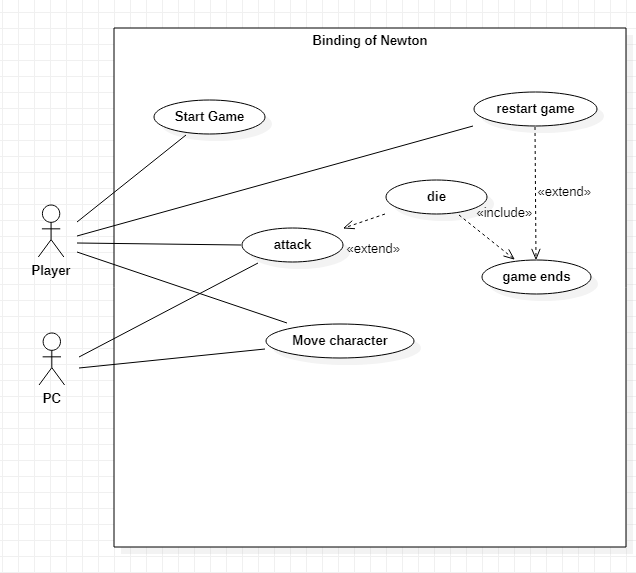
\includegraphics[scale=0.5]{case.png}
\end{figure}

\begin{figure}[H]
    \centering
    \caption{Class Diagram}
    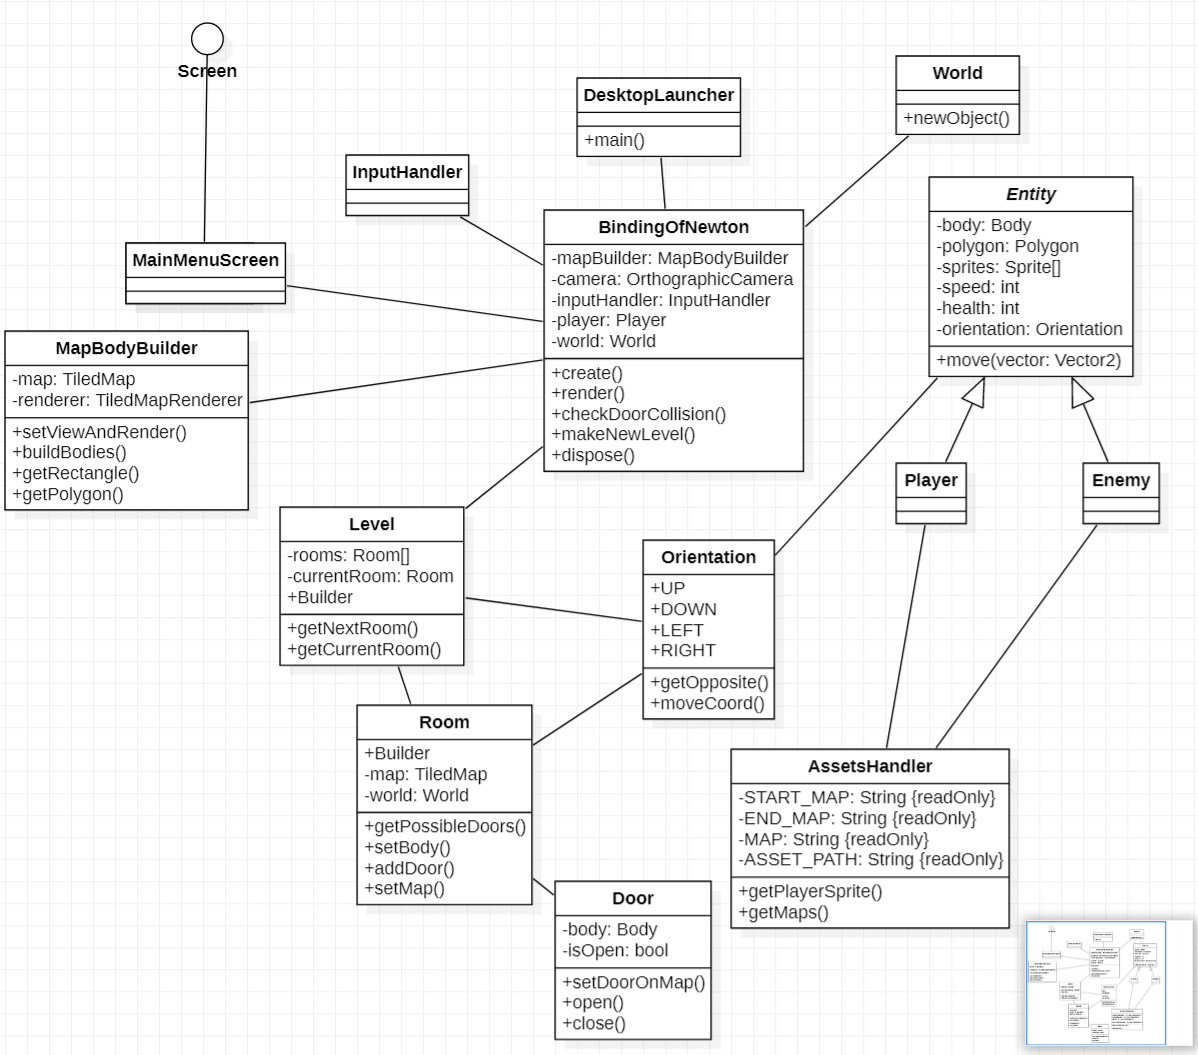
\includegraphics[scale=0.3]{class.png}
\end{figure}

\begin{figure}[H]
    \centering
    \caption{Flowchart Diagram}
    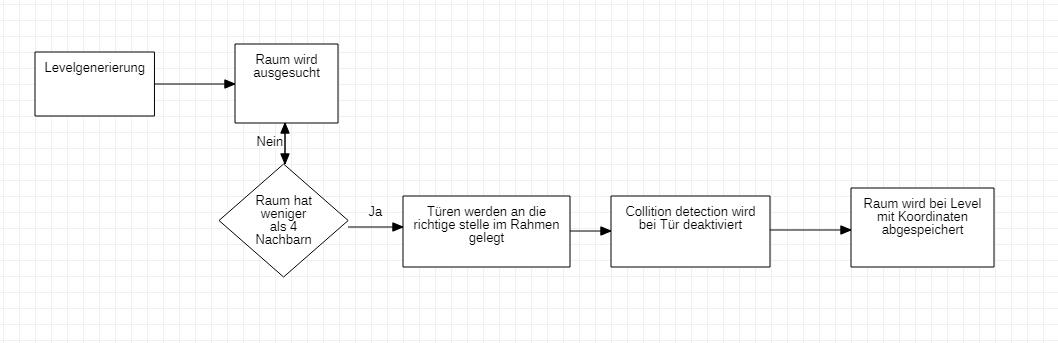
\includegraphics[scale=0.4]{flow.png}
\end{figure}

\subsection{Zeitplan}
Es wurde ein grober Zeitplan erstellt, dieser wird dynamisch erweitert. 

\subsection{TODO-Liste }
Es wurde ein Trello Board erstellt. Es gibt eine „TODO$``$ Liste, sobald die Aufgaben erledigt sind werden sie in die „Done$``$ Liste verschoben.

\section{Verweise zu anderen Dokumenten}
\begin{itemize}
	\item Mockup GUI: \\
(\url{https://www.figma.com/file/laXGb3SDypdL1TtVh45v3G/Untitled?node-id=0\%3A1}{https://www.figma.com/file/laXGb3SDypdL1TtVh45v3G/Untitled?node-id=0$\%$ 3A1})
	\item Klassendiagramm: (\url{https://github.com/PK-Sterzing/bindingofnewton/blob/main/docs/classdiagram.mdj})
	\item Use-Case Diagram: (\url{https://github.com/PK-Sterzing/bindingofnewton/blob/main/docs/Use%20Case.mdj})
	\item Alle Versionen des Zeitplans: (\url{https://github.com/PK-Sterzing/bindingofnewton/blob/main/docs/Zeitplan.xlsx})
	\item Trello Board: (\url{https://trello.com/b/vEMzPzZA/binding-of-newton})
\end{itemize}

\vspace{\baselineskip}
\printbibliography
\end{document}